\section*{Anhang}

\begin{minipage}[t]{0.4\textwidth}
    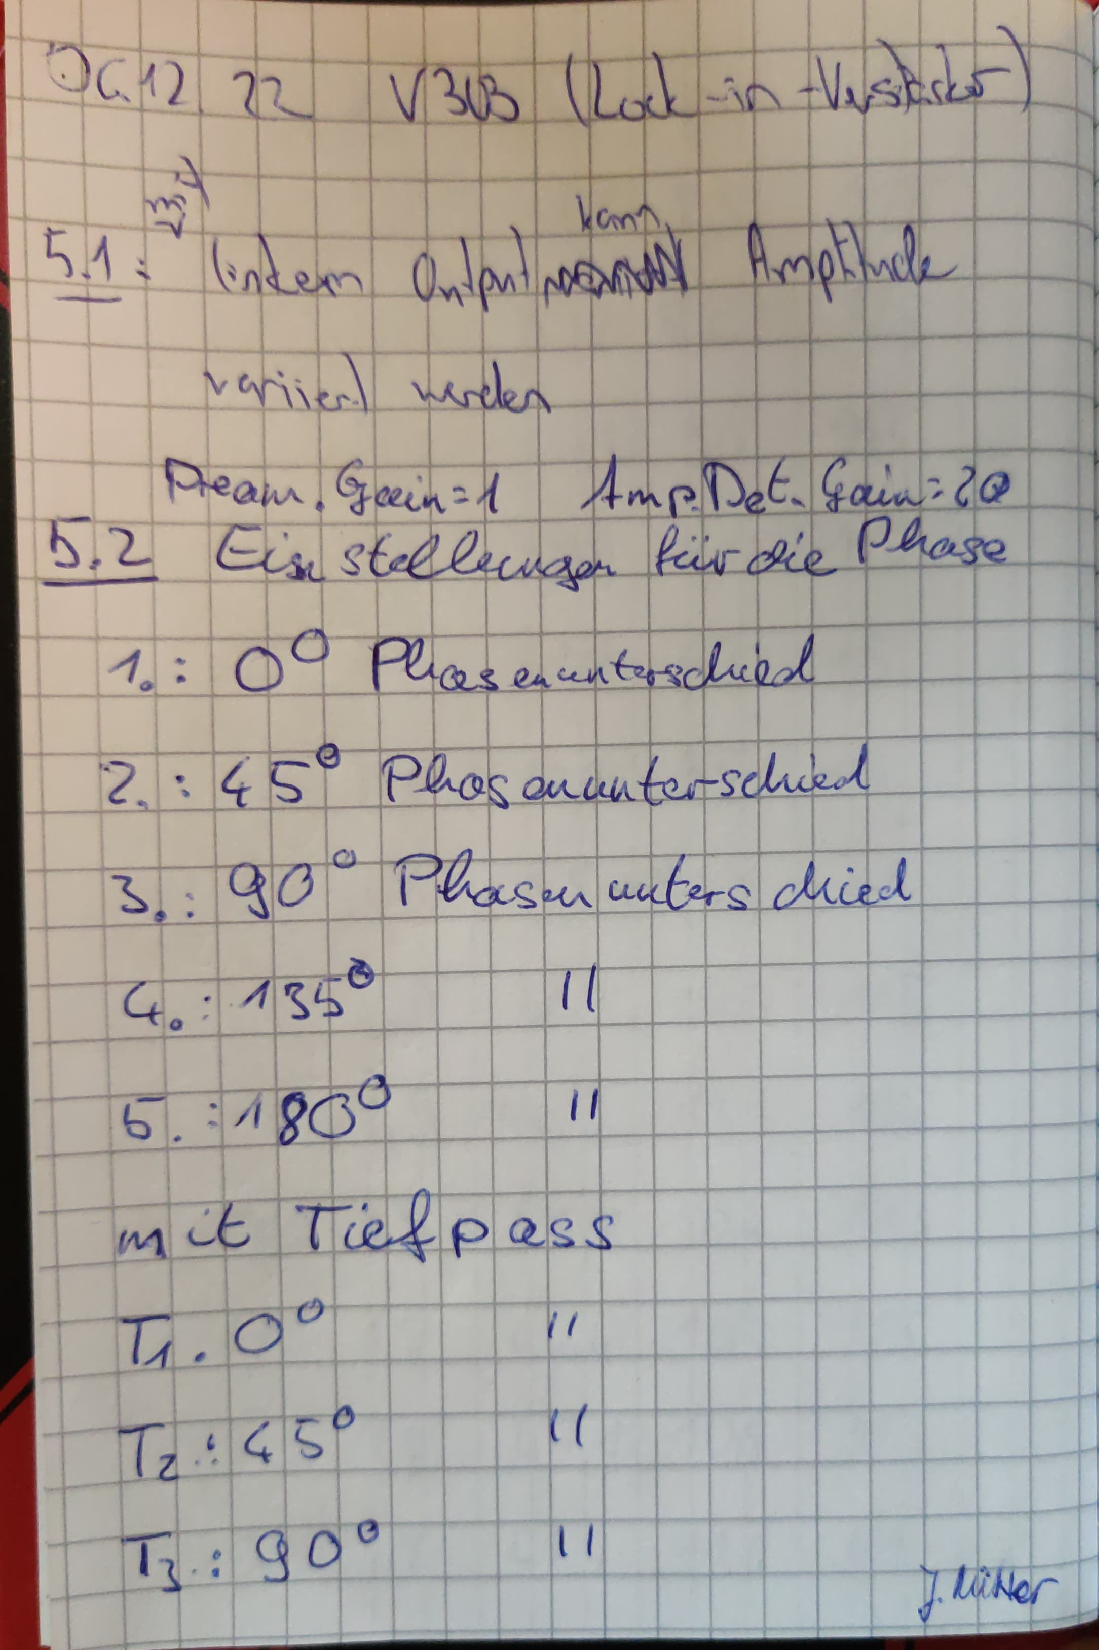
\includegraphics[width=\textwidth, page=1]{v303_messdaten.pdf}
\end{minipage}
\begin{minipage}[t]{0.4\textwidth}
    \includegraphics[width=\textwidth, keepaspectratio, page=2]{v303_messdaten.pdf}
\end{minipage}

\begin{minipage}[t]{0.4\textwidth}
    \includegraphics[width=\textwidth, page=3]{v303_messdaten.pdf}
\end{minipage}
\begin{minipage}[t]{0.4\textwidth}
    \includegraphics[width=\textwidth, page=4]{v303_messdaten.pdf}
\end{minipage}

\begin{minipage}[t]{0.4\textwidth}
    \includegraphics[width=\textwidth, page=5]{v303_messdaten.pdf}
\end{minipage}

\newpage

\begin{figure}%
    \begin{subfigure}{0.5\textwidth}%
    \centering%
    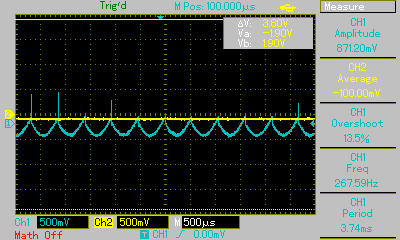
\includegraphics[width = 7.3cm]{./Oszilloskop Bilder/png/5.2/T1.png}%
    \caption{$\phi = \qty[]{0}{\degree}$}%
    %\label{fig:phase1}%
    \end{subfigure}%
    %
    \hfill% Fills available space in the center -> space between figures
    \begin{subfigure}{0.5\textwidth}%
    \centering%
    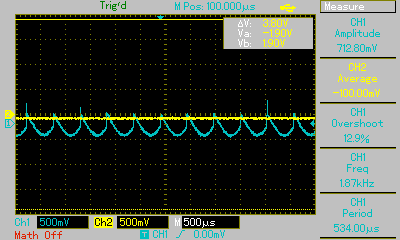
\includegraphics[width = 7.3cm]{./Oszilloskop Bilder/png/5.2/T2.png}%
    \caption{$\phi = \qty[]{45}{\degree}$}%
    %\label{fig:phase2}%
    \end{subfigure}%
    %
    \hfill
    \begin{subfigure}{0.5\textwidth}%
    \centering%
    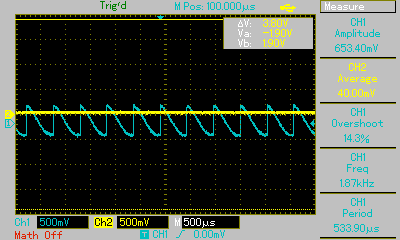
\includegraphics[width = 7.3cm]{./Oszilloskop Bilder/png/5.2/T3.png}%
    \caption{$\phi = \qty[]{90}{\degree}$}%
    %\label{fig:phase3}%
    \end{subfigure}%
    %
    \hfill% Fills available space in the center -> space between figures
    \begin{subfigure}{0.5\textwidth}%
    \centering%
    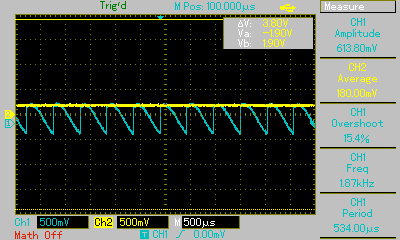
\includegraphics[width = 7.3cm]{./Oszilloskop Bilder/png/5.2/T4.png}%
    \caption{$\phi = \qty[]{135}{\degree}$}%
    %\label{fig:phase4}%
    \end{subfigure}%
    %
    \hfill
    \begin{subfigure}{0.5\textwidth}%
    \centering%
    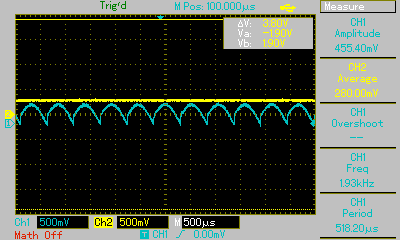
\includegraphics[width = 7.3cm]{./Oszilloskop Bilder/png/5.2/T5.png}%
    \caption{$\phi = \qty[]{180}{\degree}$}%
    %\label{fig:phase5}%
    \end{subfigure}%
    %    
    \hfill
    \begin{subfigure}{0.5\textwidth}%
    \centering%
    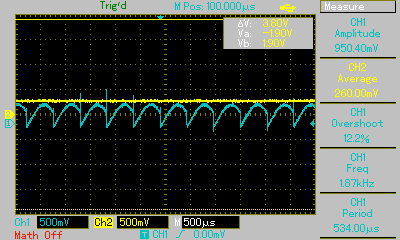
\includegraphics[width = 7.3cm]{./Oszilloskop Bilder/png/5.2/T6.png}%
    \caption{$\phi = \qty[]{225}{\degree}$}%
    %\label{fig:phase5}%
    \end{subfigure}%
    %
    \hfill
    \begin{subfigure}{0.5\textwidth}%
    \centering%
    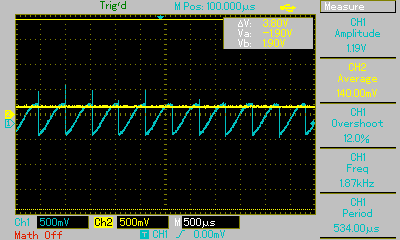
\includegraphics[width = 7.3cm]{./Oszilloskop Bilder/png/5.2/T7.png}%
    \caption{$\phi = \qty[]{270}{\degree}$}%
    %\label{fig:phase5}%
    \end{subfigure}%
    %
    \hfill
    \begin{subfigure}{0.5\textwidth}%
    \centering%
    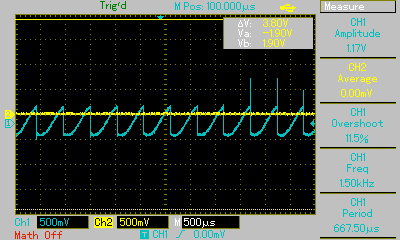
\includegraphics[width = 7.3cm]{./Oszilloskop Bilder/png/5.2/T8.png}%
    \caption{$\phi = \qty[]{315}{\degree}$}%
    %\label{fig:phase5}%
    \end{subfigure}%
    %
    \hfill
    \begin{subfigure}{0.5\textwidth}%
    \centering%
    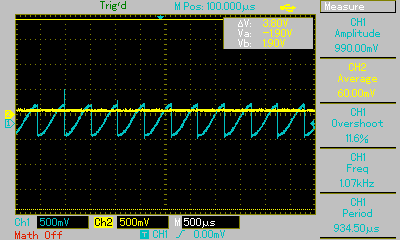
\includegraphics[width = 7.3cm]{./Oszilloskop Bilder/png/5.2/T9.png}%
    \caption{$\phi = \qty[]{300}{\degree}$}%
    %\label{fig:phase5}%
    \end{subfigure}%
    %
    \hfill
    \begin{subfigure}{0.5\textwidth}%
    \centering%
    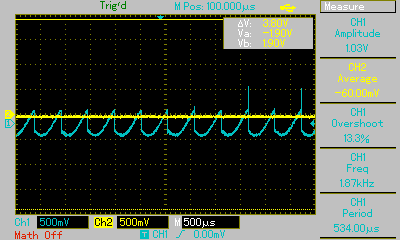
\includegraphics[width = 7.3cm]{./Oszilloskop Bilder/png/5.2/T10.png}%
    \caption{$\phi = \qty[]{315}{\degree}$}%
    %\label{fig:phase5}%
    \end{subfigure}%
    %
    \caption{Spannungsverläufe mit Tiefpass und ohne Noise Generator}%
\end{figure}%

\begin{figure}%
    \begin{subfigure}{0.5\textwidth}%
    \centering%
    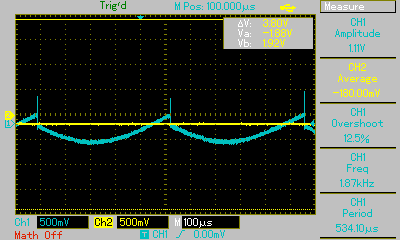
\includegraphics[width = 7.3cm]{./Oszilloskop Bilder/png/5.3/nt1.png}%
    \caption{$\phi = \qty[]{0}{\degree}$}%
    %\label{fig:phase1}%
    \end{subfigure}%
    %
    \hfill% Fills available space in the center -> space between figures
    \begin{subfigure}{0.5\textwidth}%
    \centering%
    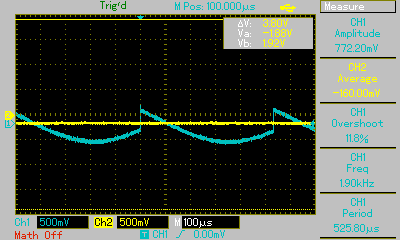
\includegraphics[width = 7.3cm]{./Oszilloskop Bilder/png/5.3/nt2.png}%
    \caption{$\phi = \qty[]{45}{\degree}$}%
    %\label{fig:phase2}%
    \end{subfigure}%
    %
    \hfill
    \begin{subfigure}{0.5\textwidth}%
    \centering%
    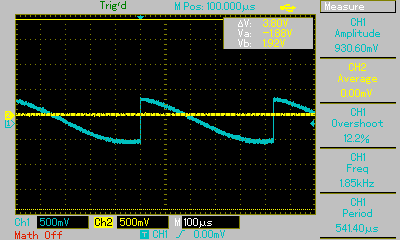
\includegraphics[width = 7.3cm]{./Oszilloskop Bilder/png/5.3/nt3.png}%
    \caption{$\phi = \qty[]{90}{\degree}$}%
    %\label{fig:phase3}%
    \end{subfigure}%
    %
    \hfill% Fills available space in the center -> space between figures
    \begin{subfigure}{0.5\textwidth}%
    \centering%
    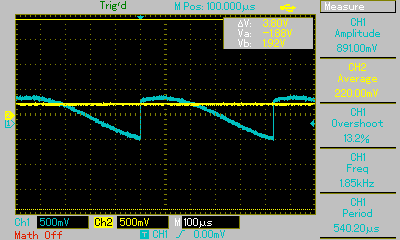
\includegraphics[width = 7.3cm]{./Oszilloskop Bilder/png/5.3/nt4.png}%
    \caption{$\phi = \qty[]{135}{\degree}$}%
    %\label{fig:phase4}%
    \end{subfigure}%
    %
    \hfill
    \begin{subfigure}{0.5\textwidth}%
    \centering%
    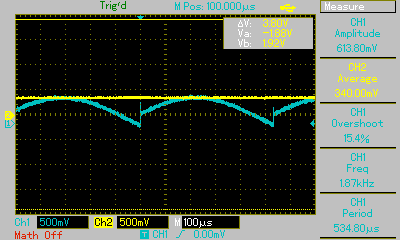
\includegraphics[width = 7.3cm]{./Oszilloskop Bilder/png/5.3/nt5.png}%
    \caption{$\phi = \qty[]{180}{\degree}$}%
    %\label{fig:phase5}%
    \end{subfigure}%
    %    
    \hfill
    \begin{subfigure}{0.5\textwidth}%
    \centering%
    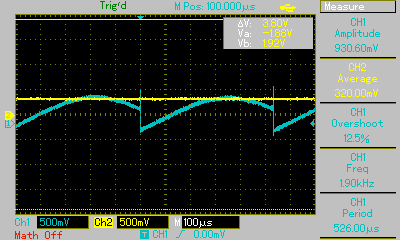
\includegraphics[width = 7.3cm]{./Oszilloskop Bilder/png/5.3/nt6.png}%
    \caption{$\phi = \qty[]{225}{\degree}$}%
    %\label{fig:phase5}%
    \end{subfigure}%
    %
    \hfill
    \begin{subfigure}{0.5\textwidth}%
    \centering%
    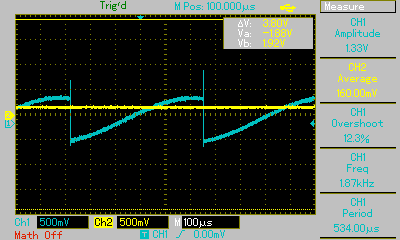
\includegraphics[width = 7.3cm]{./Oszilloskop Bilder/png/5.3/nt7.png}%
    \caption{$\phi = \qty[]{270}{\degree}$}%
    %\label{fig:phase5}%
    \end{subfigure}%
    %
    \hfill
    \begin{subfigure}{0.5\textwidth}%
    \centering%
    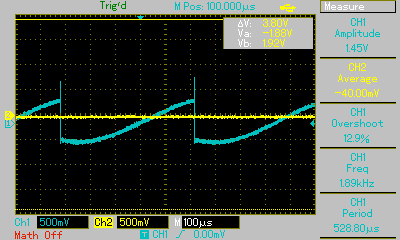
\includegraphics[width = 7.3cm]{./Oszilloskop Bilder/png/5.3/nt8.png}%
    \caption{$\phi = \qty[]{315}{\degree}$}%
    %\label{fig:phase5}%
    \end{subfigure}%
    %
    \hfill
    \begin{subfigure}{0.5\textwidth}%
    \centering%
    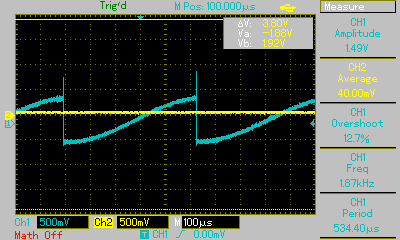
\includegraphics[width = 7.3cm]{./Oszilloskop Bilder/png/5.3/nt9.png}%
    \caption{$\phi = \qty[]{300}{\degree}$}%
    %\label{fig:phase5}%
    \end{subfigure}%
    %
    \hfill
    \begin{subfigure}{0.5\textwidth}%
    \centering%
    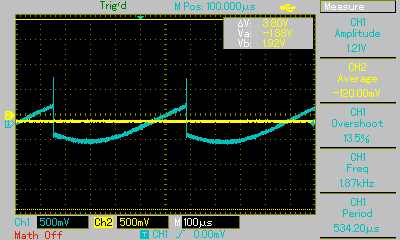
\includegraphics[width = 7.3cm]{./Oszilloskop Bilder/png/5.3/nt10.png}%
    \caption{$\phi = \qty[]{315}{\degree}$}%
    %\label{fig:phase5}%
    \end{subfigure}%
    %
    \caption{Spannungsverläufe mit Tiefpass und mit Noise Generator}%
\end{figure}%
